\section{FORM OPTIMIZATION BASED ON FLIGHT STABILITY}
\subsection{Optimal Form Based on Flight Stability}
The dynamics of the model is described is \equref{P}. Therefore, when the control system is at steady state, the control model can be written as follows:
\begin{equation}
  P(\bm{\theta}, m_{obj}, \bm{r}_{obj})\bm{u}=\bm{G}
  \label{eq:steady_state}
\end{equation}
where $\bm{\theta}$, $m_{obj}$ and $\bm{r}_{obj}$ denotes the angle vector of joints ($\theta_1, \cdots, \theta_N$), the mass and the position of a object which the multirotor grasps respectively to emphasize that matrix $P$ is influenced by them.
\par
When any element in $\bm{u}$ exceeds the range of lifting forces, the flight control is unstable. Although all elements of $\bm{u}$ fall within the range of forces, any one of them can exceed the range of forces when it is close to the upper limit of forces due to the flight control and disturbance. Hence, the most stable state is that all elements of $\bm{u}$ are equal since the sum of $\bm{u}$ equal to $MG$ which is constant at the steady state. This is written as:
\begin{equation}
  \text{min} V(\bm{u}) \ \text{subject to} \ P\bm{u}=\bm{G}
  \label{eq:optimization}
\end{equation}
where the function $V(x)$ is used to calculate the variance of elements of $x$. 
\par
This variance can be written as:
\begin{equation}
  V(\bm{u})=E(\bm{u}^2)-E(\bm{u})^2
\end{equation}
where the function $E(x)$ is used to calculate the mean of elements of $x$. 
\par
Note that $E(\bm{u})^2$ is a constant term since the sum of $\bm{u}$ is equal to $MG$ at steady state.
\par
Hence, the problem in \equref{optimization} can be redefined as:
\begin{equation}
  \text{min}\bm{u}^\mathrm{T}\bm{u} \ \text{subject to} \ P\bm{u}=\bm{G}
  \label{eq:optimization2}
\end{equation}
When $N=4$ and P is full rank, \equref{steady_state} can be solved as $\bm{u}=P^{-1}\bm{G}$. However, for a system with more than four links, a null space occurs, resulting in an infinite solution for $\bm{u}$. In this case, we use Lagrange multiplier to obtain least-norm solution of $\bm{u}$ since the purpose is to minimize the norm of $\bm{u}$ as shown in \equref{optimization2}. 
\par
The Lagrange multiplier can be written as:
\begin{equation}
  \bm{u}=P(PP^\mathrm{T})^{-1}\bm{G}
  \label{eq:P_inv}
\end{equation}

\subsection{Constraints of Form of Multilinks}
 Even though the optimal form can be obtained as described in \equref{optimization2}, the solution can be invalid. Therefore, the solution must satisfy constraints to avoid invalid forms. Five constraints are shown as follows.
\subsubsection{Joint Angle Limit}
In this work, the rotation range of each joint is $-\frac{\pi}{2}$[rad] $\sim$ $\frac{\pi}{2}$[rad]. The joint angles must be changed in this range since a command of joint angle which is out of this range does not make sense.
\subsubsection{Self-Collision}
Although the joint angles are in the range, self-collision can occur as shown in \figref{invalid_forms}(a). Therefore, collision detection is necessary to avoid self-collision.
\subsubsection{Rank of P}
According to \equref{P}, if $P$ has full rank, the mapping is surjective, indicating that the four elements in $\bm{y} \ (z,\varphi, \theta, \psi)$ are dependent of each other. In contrast, if $P$ is not of full rank, the four elements can not act independently, leading to an uncontrollable result. We call the resulting special form the singular form(\figref{invalid_forms}(b)).The rank of P can be calculated by checking the linear combination of row vectors $(\bm{\mathrm{p}}_z , \bm{\mathrm{p}}_x , \bm{\mathrm{p}}_y , \bm{\mathrm{p}}_c )$. %It is evident that $\bm{\mathrm{p}}_z$ and $\bm{\mathrm{p}}_c$ are linearly independent, and the linear independence of the two group ($\{\bm{\mathrm{p}}_z, \bm{\mathrm{p}}_x , \bm{\mathrm{p}}_y \}$ and $\{\bm{\mathrm{p}}_c , \bm{\mathrm{p}}_x , \bm{\mathrm{p}}_y \}$) must be checked. 
When the multirotor is under the singular form, its control system is asymptotically unstable.
\subsubsection{Lifting Force Range}
Lifting force which is generated by the propeller has the range. In the case of our own machine, the range of lifting force is (0[N]$\sim$16.5[N]). All elements of the input vector $\bm{u}$ in \equref{P_inv} must fall within this range of forces.
\subsubsection{Distance from Each Propeller to the Rotational Axis}
There can be unavoidable errors in the control model(\equref{P}) and state equation(\equref{state_eq}) because of estimation errors in the inertia parameters. The most serious error concerns the estimation of $x_i$ and $y_i$ as shown in \figref{dynamic_model}. The distance $x_i$, $y_i$ has a significant effect on the moment for pitch and roll rotation, especially when all elements in $x$ or $y$ are close to zero, in which case the estimation error can assign the wrong sign of $x_i$, $y_i$, producing a roll/pitch moment in the wrong direction.
\par
To avoid this, it is necessary to keep the distance $x_i$, $y_i$ large enough. We, therefore, introduce the following distance indices $d_x$, $d_y$ to evaluate each state:
\begin{equation}
  \begin{cases}
    \; d_x(\text{\it{State}}(\bm{\theta})) = \frac{\min(|\min(\bm{x}(\bm{\theta}))|,\max(\bm{x}(\bm{\theta})))}{r}\\
    \; d_y(\text{\it{State}}(\bm{\theta})) = \frac{\min(|\min(\bm{y}(\bm{\theta}))|,\max(\bm{y}(\bm{\theta})))}{r}\\
  \end{cases}
  \label{eq:dx_dy}
\end{equation}
\par
We then use the indices to validate the state in terms of the distance of pitch/roll moment, using a thresholding method as follows:
\begin{equation}
  \begin{split}
  %\text{\it{Validator_{dist}}}(\text{\it{State}}(\bm{\theta}))=\\                                                                                                        
  \text{\it{Validator}}_{dist}(\text{\it{State}}(\bm{\theta}))= \hspace{0.4\columnwidth} \\
  \begin{cases}
  \text{\it{Valid}} \hspace{0.2\columnwidth}(d_x(\text{\it{State}}(\bm{\theta})) >= \text{\it{Threshold}} \\
  \hspace{0.2\columnwidth} \text{\it{AND}} \ d_y(\text{\it{State}}(\bm{\theta})) >= \text{\it{Threshold}})\\
  \text{\it{Invalid}} \hspace{0.2\columnwidth} (d_x(\text{\it{State}}(\bm{\theta})) < \text{\it{Threshold}} \\ 
  \hspace{0.2\columnwidth} \text{\it{OR}} \ d_y(\text{\it{State}}(\bm{\theta})) < \text{\it{Threshold}})
  \end{cases}
  \end{split}
  \label{eq:dx_dy_thresh}
\end{equation}
\par
The target state will be validated as an invalid state, if either of the two indices fall below the threshold. The form shown in \figref{invalid_forms}(c) is an example of an invalid state.

\begin{figure}[th]
  \begin{center}
    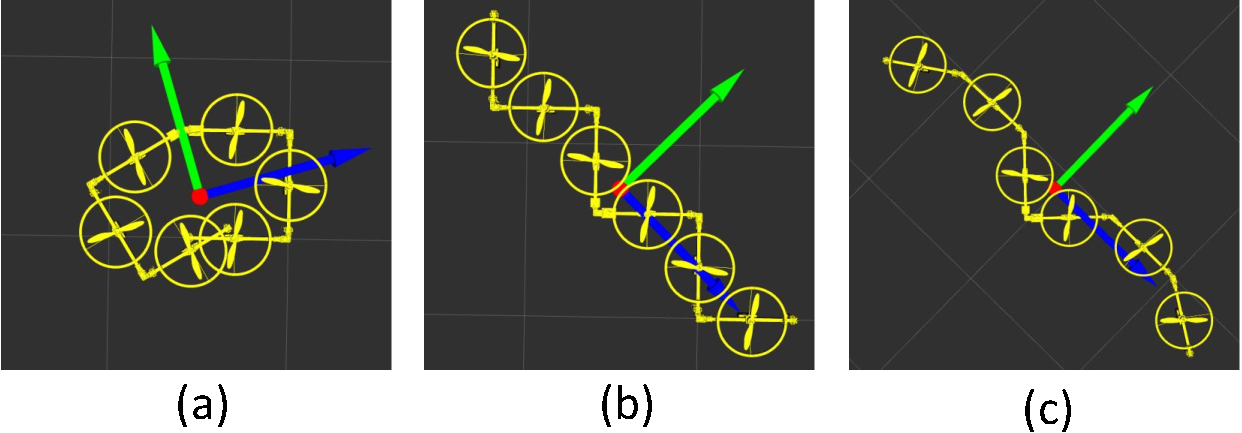
\includegraphics[width=1.0\columnwidth]{figs/invalid_forms.pdf}
  \end{center}
  \caption{Examples of invalid forms. \newline
(a): Self-collision form($\theta_1=\theta_2=\theta_4=\theta_5=\frac{\pi}{2}$[rad], $\theta_3=0.55$[rad]). \newline (b): Singular form($\theta_1=\theta_3=\theta_5=\frac{\pi}{2}$[rad], $\theta_2=\theta_4=-\frac{\pi}{2}$[rad]). \newline (c): Invalid form based on roll/pitch moment($\theta_1=\theta_5=0.80$[rad], $\theta_2=\theta_4=0.57$[rad], $\theta_3=-\frac{\pi}{2}$[rad]).\label{figure:invalid_forms}}
\end{figure}

\begin{figure}[th]
  \begin{center}
    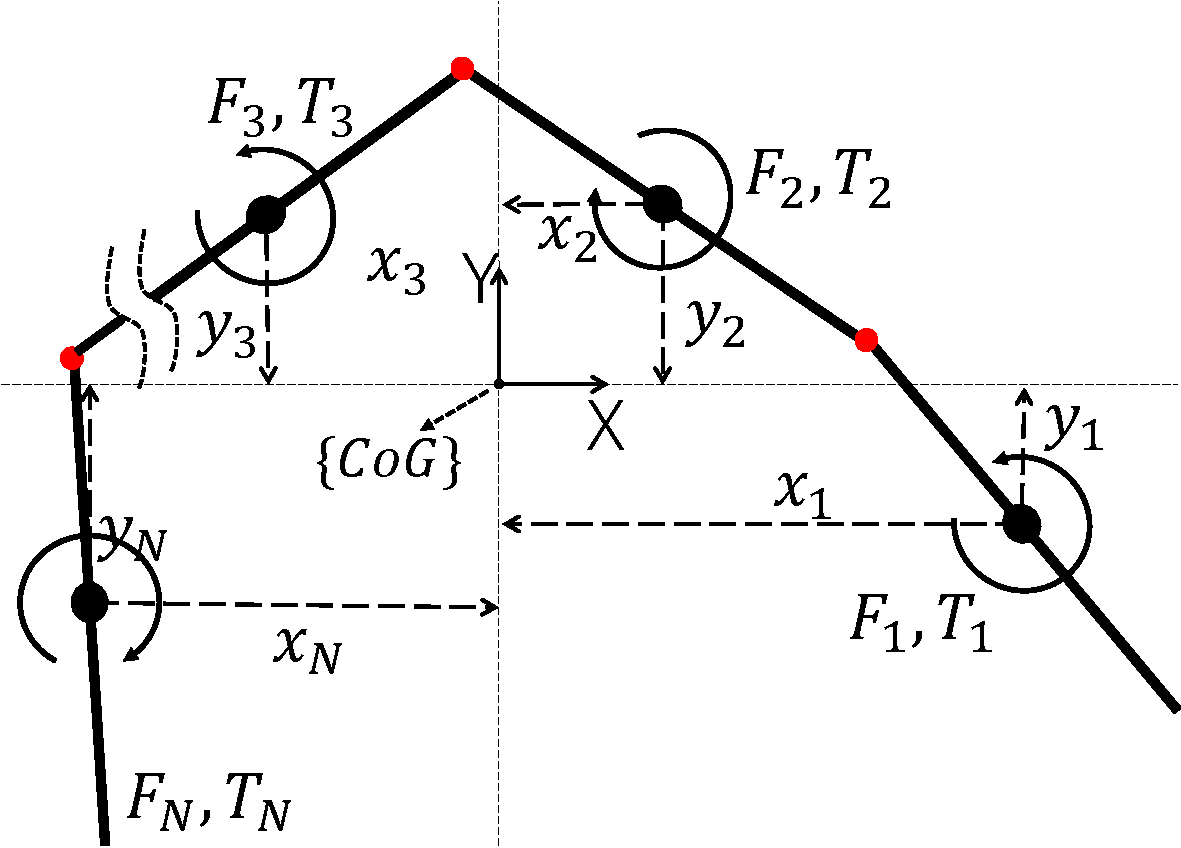
\includegraphics[width=0.9\columnwidth]{figs/dynamic_model.pdf}
    \caption{The dynamic model of the quadrotor prototype described in coordinate frame $\{CoG\}$. $F_i$ and $T_i$ denote the lifting force and torque generated by each propeller, respectively. $[x_i, y_i]$ is the location of each propeller in the frame of $\{CoG\}$.\label{figure:dynamic_model}}
  \end{center}
\end{figure}

\subsection{Optimal Form Based on Gradient Descent}
To determine the joint angle vector $\bm{\theta}$ which minimizes $\bm{u}^\mathrm{T}\bm{u}$(\equref{optimization2}, \equref{P_inv}), we apply gradient descent(steepest descent)\cite{OZEKI2003}. In gradient descent, the joint angle vector $\bm{\theta}$ is updated as follows:
\begin{equation}
  \bm{\theta}^{(k+1)} = \bm{\theta}^{(k)}-\alpha \ \text{grad}(F(\bm{\theta}^{(k)}))
  \label{eq:steepest_descent_method}
\end{equation}
\begin{equation*}
  F(\bm{\theta})=\bm{u}(\bm{\theta})^\mathrm{T}\bm{u}(\bm{\theta})
\end{equation*}
Note that $\alpha$ is a parameter which determines the weight of one update and is normally defined as small positive value. Although $F$ is necessary to be differentiable, it is a simple method since only first derivative must be calculated. In this work, as it is difficult to calculate partial derivative of $F$, instead of this, we calculate variation of $F$. This is written as:
\begin{equation}
  \text{grad}(F(\bm{\theta}))_i=\frac{F(\bm{\theta}+\Delta \bm{\theta_i})-F(\bm{\theta})}{\Delta \theta}
  \label{eq:grad}
\end{equation}
where $\Delta \theta$ and $\Delta \bm{\theta_i}$ are infinitesimal angle and column vector whose i-th component is $\Delta \theta$ and the other components are 0, respectively. We also introduce $V_{th}$, the lower limit of $V(\bm{u})$ as a termination condition of optimization. Since the upper limit of lifting force is 16.5[N] in the case of our own machine, we set $V_{th}$ to 0.001[$\text{N}^2$]. In other words, we stop the optimization when $V(\bm{u})$ is 0.001[$\text{N}^2$] since the value can be considered to be converged fully. Besides, since the solution obtained by gradient descent depends on the initial value, there is a possibility that valid solution is not obtained. Accordingly, we perform optimization with multiple initial values($\theta_i = 0.0, 0.1, \cdots, 1.0$). 
\par
Then, setting parameters of gradient descent as shown in \tabref{optimization_params}, we perform optimization calculation on four conditions shown in \figref{optimization_result}. In \figref{optimization_result}(a) $\sim$ \figref{optimization_result}(d), the orange circle indicates the position of the additional mass(0.5[kg]) while the red circle and the blue, green arrows indicate the position of CoG and principal axes of inertia, respectively. According to the final values of $V(\bm{u})$ shown under each form, it is evident that the optimization is fully performed and optimal forms can be obtained by this method.

\begin{table}[th]
 \caption{Parameters of gradient descent.}
 \label{table:optimization_params}
 \centering
 \begin{tabular}{|p{7zw}|l|l|l|}
  \hline
  parameter & value & description \\ \hline \hline
  $\alpha$ & 0.3 & weight of update[$\text{rad}^2/\text{N}^2$]\\
  $m_{UAV}$ & 5 & UAV mass[kg]\\
  $m_{obj}$ & 0.5 & additional mass[kg]\\
  $V_{th}$ & 0.001 & lower limit of $V(\bm{u})$[$\text{N}^2$]\\
  \hline
 \end{tabular}
\end{table}

\begin{figure}[H]
  \begin{center}
    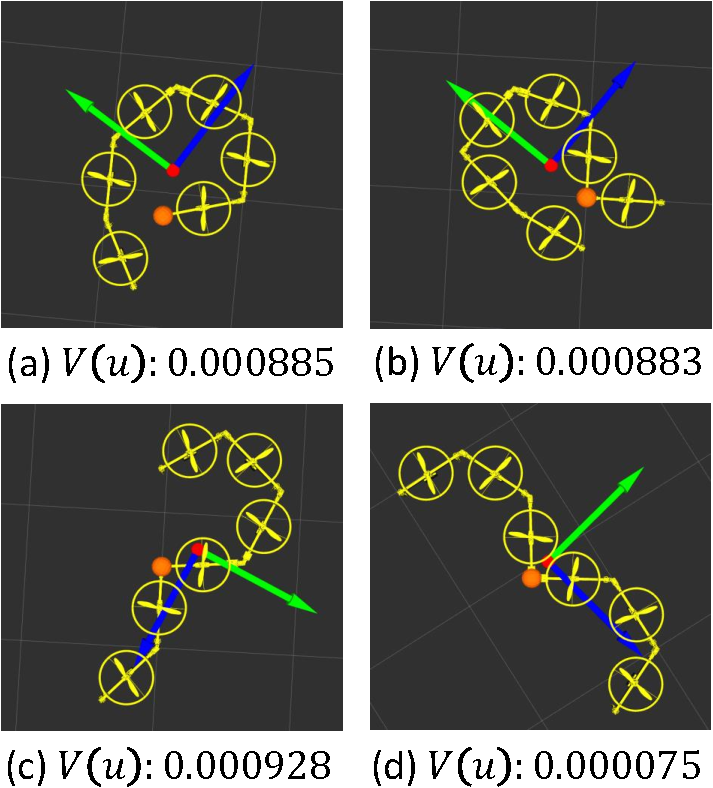
\includegraphics[width=0.8\columnwidth]{figs/optimization_result.pdf}
    \caption{The optimized forms of each case with gradient descent: the values under each form is the final value of $V(\bm{u})$. \label{figure:optimization_result}}
  \end{center}
  
\end{figure}
